\documentclass{article}

\usepackage[a4paper, total={6.5in, 11in}]{geometry}
\usepackage{graphicx}
\usepackage{subfig}
\usepackage{gensymb}
\usepackage{hyperref}
\graphicspath{{titech/CSC.T463.ComputerGraphics/h5/}}

\usepackage{latex/common}

\title{Computer Graphics 2021 - Assignment 5}
\author{Sixue Wang\\21M30927\\Tokyo Institute of Technology}

\begin{document}

\maketitle

\section{}

We can calcuate CIEXYZ1931 coordinate by the following equtions:

\begin{equation}
   X =  \int_{\lambda} S(\lambda)\frac{PlanckEquation(\lambda)}{PlanckEquation(590e-9)} x(\lambda) d\lambda
\end{equation}
\begin{equation}
   Y =  \int_{\lambda} S(\lambda)\frac{PlanckEquation(\lambda)}{PlanckEquation(590e-9)} y(\lambda) d\lambda
\end{equation}
\begin{equation}
   Z =  \int_{\lambda} S(\lambda)\frac{PlanckEquation(\lambda)}{PlanckEquation(590e-9)} z(\lambda) d\lambda
\end{equation}
Furthermore, we can normalize them by $\int_{\lambda} \frac{PlanckEquation(\lambda)}{PlanckEquation(590e-9)} y(\lambda) d\lambda$

\section{}
To calcuate sRGB coordinate, we transform tristimulus values by the following matrix
\begin{equation}
  \begin{bmatrix}
    R \\ G \\ B
  \end{bmatrix}
  =
  \begin{bmatrix}
    3.2406  & -1.5372 & -0.4986 \\
    -0.9689 & 1.8758  & 0.0415  \\
    0.0557  & -0.2040 & 1.0570
  \end{bmatrix}
  \begin{bmatrix}
    X \\ Y \\ Z
  \end{bmatrix}
\end{equation}
Then process RGB one by one as following method:
\begin{equation}
  if \; RGB < 0.0031308 \; then \;
    RGB *= 12.92 \;
  else \;
    RGB = 1.055 * RGB^{\frac{1}{2.4}} - 0.055
\end{equation}
We also use \href{https://github.com/colour-science/colour}{colour}(a python tool) to verify our answer.


\includegraphics[width=\textwidth]{h5_1.png}

\section{}
Personally, I think there is only one brightest and one darkest pigment in the D65 illumination condition. In CIEXYZ, Y is known as the relative luminance which can represent the brightness. We can show $\frac{PlanckEquation(\lambda)}{PlanckEquation(590e-9)} y(\lambda)$

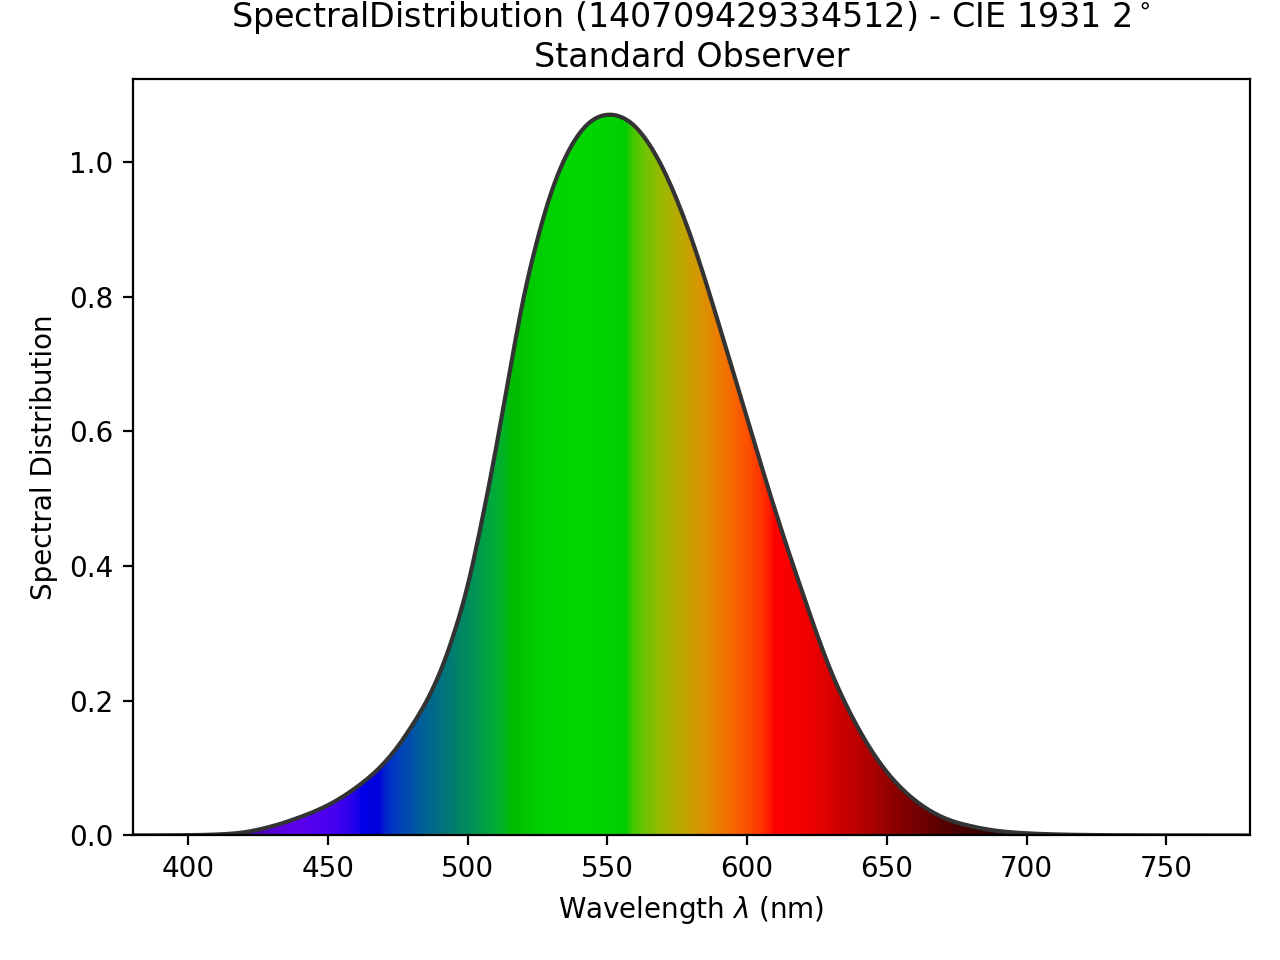
\includegraphics{h5_2.png}

\end{document}
